\chapter{Evaluation}\label{chap:eval}

% Least Squares Linear Regression
% p73 onwards https://people.cs.uchicago.edu/~mrocklin/storage/dissertation.pdf

% \begin{guidance}
%     For any practical projects, you should almost certainly have
%     some kind of evaluation, and it's often useful to separate
%     this out into its own chapter.
% \end{guidance}

\prechapter{%
    I will evaluate the central premise of this thesis: linear types are a
    practical and usable tool to help programmers write readable (equational
    and algebraic), safe (with respect to aliasing, read/write permissions,
    memory re-use and deallocation) and explicit (with respect to memory
    allocation) code that (1) is more memory-efficient than code written using
    high-level linear algebra libraries and (2) performs just as predictably as
    code written using low-level linear-algebra libraries. I will also
    elaborate on the qualitative benefits of using linear types to write
    linear-algebra programs.
}%

\section{Compared to C}

To test whether code written using LT4LA performs just as predictably as code
written using low-level linear-algebra libraries, I wrote two implementations
of a Kalman filter:

\begin{enumerate}

    \item A CBLAS/LAPACKE implementation, written in C
        (Figure~\ref{fig:cblas_kalman}), with a minimal number of temporaries,
        calls to `symm' for matrices known to be symmetric ahead of time,
        transposition passed in to `gemm' as a flag and Cholesky decomposition
        for multiplying by an inverse of a matrix.

    \item A LT4LA implementation (Figure~\ref{fig:ltfla_kalman}), also with a
        minimal number of temporaries, calls to `symm' for matrices known to be
        symmetric ahead of time, transposition passed in to `gemm' as a flag
        and Cholesky decomposition for multiplying by an inverse of a matrix.

\end{enumerate}

Both implementations produce the same answers (within at most $2^{-52}$). Raw
output of implementation traces and the benchmarking program (including sample
sizes) are in Appendix~\ref{chap:eval_data}.

I compared the implementations on two metrics: memory usage (via number and
size of temporaries allocated) and execution time. For the former, I compiled
Owl with print-statements on the relevant primitives to see exactly the number
of temporaries allocated for a single call of each function. While I did also
attempt to use gperftools and OCaml's profiling support with gprof for a more
holistic view of memory usage in the presence of OCaml's garbage-collector, I
ran into technical difficulties irrelevant to this thesis.

I measured execution time, in micro-seconds, against an exponentially (powers
of 5) increasing scaling factor for matrix size parameters $n=5$ and $k=3$.
For small scaling factors (1, 5, 25), I used the Core\_bench micro-benchmarking
library, for larger factors (125 and greater), I used the \texttt{getrusage}
system call (called \ltfla{Unix.times} in OCaml), sandwiched between calls to
\ltfla{Gc.full_major} to ensure no garbage collection took place during the
measurements.  Core\_bench performs a linear-regression (here, time against
batch-size) so includes 95\% confidence-interval with $R^2$. Larger scales have
errors reported to $\pm \sigma$ (one standard-deviation).

\subsection{Memory Usage}

Inspecting the trace for LT4LA shows 6 calls to `empty' (function for
allocating new matrices): 4 temporaries plus 2 for storing the results. From
the CBLAS implementation (Figure~\ref{fig:cblas_kalman}), we can see that it
too has 6 calls to malloc: 4 temporaries plus 2 to storing the results.

\begin{landscape}
\begin{figure}[p]
    \centering
    \begin{minipage}{1.45\textheight}
    \begin{minted}[linenos, fontsize=\small]{c}
static void kalman( const int n,               const int k,                const double *sigma, /* n,n */
                    const double *h, /* k,n */ const double *mu, /* n,1 */ double *r,           /* k,k */
                    double *data,    /* k,1 */ double **ret_mu,  /* k,1 */ double **ret_sigma   /* n,n */ ) {
        double* k_by_n = (double *) malloc(k * n * sizeof(double));
/*16*/  cblas_dsymm(CblasRowMajor, CblasRight, CblasUpper, k, n, 1., sigma, n, h, n, 0., k_by_n, n);
/*17*/  cblas_dgemm(CblasRowMajor, CblasNoTrans, CblasTrans, k, k, n, 1., k_by_n, n, h, n, 1., r, k);
/*18*/  cblas_dgemm(CblasRowMajor, CblasNoTrans, CblasNoTrans, k, 1, n, 1., h, n, mu, 1, -1., data, 1);
/*19*/  cblas_dcopy(k * n, h, 1, k_by_n, 1);
        double* k_by_k = (double *) malloc(k * k * sizeof(double));
/*20*/  cblas_dcopy(k * k, r, 1, k_by_k, 1);
/*21*/  LAPACKE_dposv(LAPACK_ROW_MAJOR, 'U', k, n, k_by_k, k, k_by_n, n);
/*23*/  LAPACKE_dpotrs(LAPACK_ROW_MAJOR, 'U', k, 1, k_by_k, k, data, 1);
        free(k_by_k);
        double* n_by_n = (double *) malloc(n * n * sizeof(double));
/*24*/  cblas_dgemm(CblasRowMajor, CblasTrans, CblasNoTrans, n, n, k, 1., h, n, k_by_n, n, 0., n_by_n, n);
        free(k_by_n);
        double* n_by_1 = (double *) malloc(n * sizeof(double));
/*25*/  cblas_dgemm(CblasRowMajor, CblasTrans, CblasNoTrans, n, 1, k, 1., h, n, data, 1, 0., n_by_1, 1);
        double* new_mu = (double *) malloc(n * sizeof(double));
/*26*/  cblas_dcopy(n, mu, 1, new_mu, 1);
/*27*/  cblas_dsymm(CblasRowMajor, CblasLeft, CblasUpper, n, 1, 1., sigma, n, n_by_1, 1, 1., new_mu, 1);
        free(n_by_1);
        double* n_by_n2 = (double *) malloc(n * n * sizeof(double));
/*28*/  cblas_dsymm(CblasRowMajor, CblasRight, CblasUpper, n, n, 1., sigma, n, n_by_n, n, 0., n_by_n2, n);
/*29*/  cblas_dcopy(n*n, sigma, 1, n_by_n, 1);
/*30*/  cblas_dsymm(CblasRowMajor, CblasLeft, CblasUpper, n, n, -1., sigma, n, n_by_n2, n, 1., n_by_n, n);
        free(n_by_n2);
        *ret_sigma = n_by_n;
        *ret_mu = new_mu; }
    \end{minted}
    \caption{CBLAS/LAPACKE implementation of a Kalman filter. I used C instead
        of Fortran because it is what Owl uses under the hood and OCaml FFI
        support for C is better and easier to use than that for Fortran. A distinct
        `measure\_kalman' function that sandwiches a call to this function with
        \texttt{getrusage} is omitted for brevity.}\label{fig:cblas_kalman}

    \end{minipage}
\end{figure}
\end{landscape}

\subsection{Execution Time}

A graph of the execution times (with error bars which are present but quite
small) is shown in Figure~\ref{fig:timings}.

\begin{figure}[t]
    \centering
    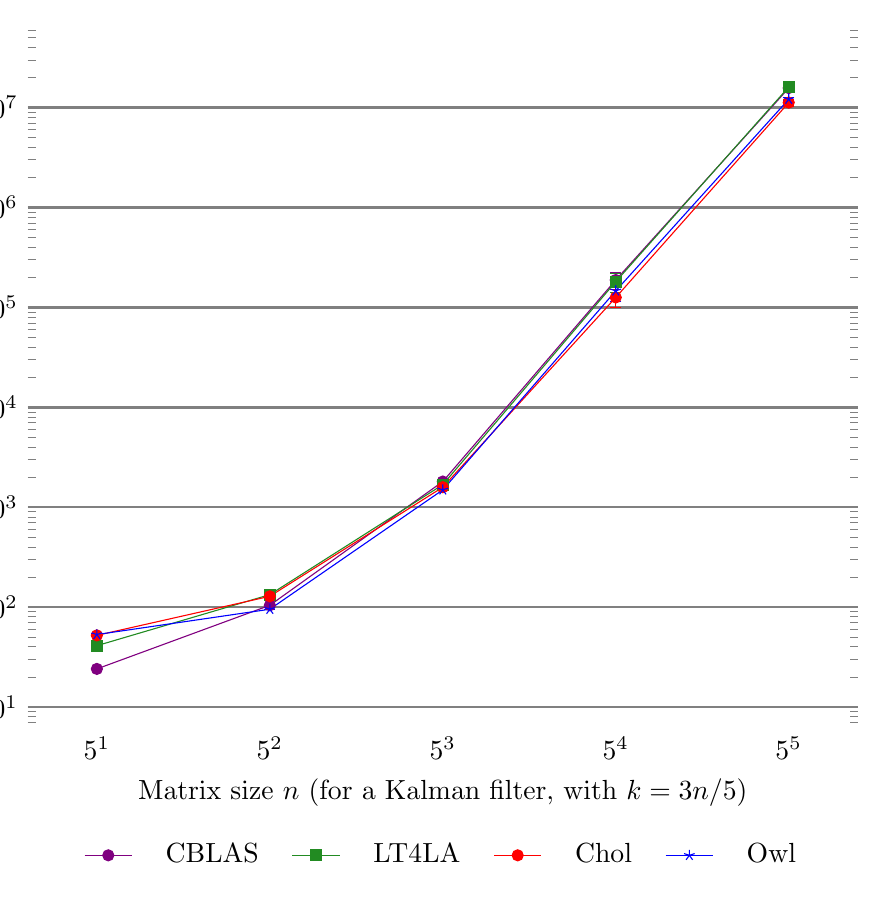
\begin{tikzpicture}[trim axis left]
\begin{axis}[
    % width of chart
    width=\textwidth,
    % no box, below chart, horizontal
    legend style={%
      draw=none,
      at={(0.5,-0.15)},
      anchor=north,
      legend columns=4,
      column sep = 1em,
      cells={align=center},
    },
    % log ticks with fixed point,
    % yticklabel={\pgfmathparse{pow(10,\tick-3)}\pgfmathprintnumber[fixed]{\pgfmathresult}}\,ms, % N ms along y-axis
    % xticklabel={\pgfmathparse{pow(5,\tick)}\pgfmathprintnumber[fixed]{\pgfmathresult}},
    xlabel near ticks,
    xlabel={Matrix size $n$ (for a Kalman filter, with $k=3n/5$)},
    ylabel near ticks,
    ylabel={Execution time of one call to Kalman filter ($\mu$s)},
    xmode = log,
    log basis x = {5},
    axis line style={opacity=0}, % hide y axis
    major tick style={draw=none}, % no ticks
    ymode=log, % log scale for y
    log basis y = {10}, % log base 10
    ymajorgrids, % rows of lines
    major grid style={gray, line width=1pt},
]

  % CBLAS
    \addplot+ [
        violet,
        mark options={fill=violet},
        error bars/.cd, y dir=both, y explicit,
    ] table [
        y error plus=ey+,
        y error minus=ey-,
    ] {
         x         y     ey+     ey-
         5        24       0       0
        25       104       1       1
       125      1803      64      57
       625    187667   36281   36281
      3125  15651064  530675  530675
  };

  % LT4LA
    \addplot+ [
        ForestGreen,
        mark options={fill=ForestGreen},
        error bars/.cd, y dir=both, y explicit,
    ] table [
        y error plus=ey+,
        y error minus=ey-,
    ] {
         x         y     ey+     ey-
         5        41       1       1
        25       133       2       2
       125      1678      36      33
       625    180575   38386   38386
      3125  16061291  193746  193746
  };

  % Chol
    \addplot+ [
        red,
        mark options={fill=red},
        error bars/.cd, y dir=both, y explicit,
    ] table [
        y error plus=ey+,
        y error minus=ey-,
    ] {
         x         y     ey+     ey-
         5        52       1       1
        25       128       1       1
       125      1583      95      75
       625    125526   25502   25502
      3125  11210982 852463   852463
  };

  % Owl
    \addplot+ [
        Blue,
        mark options={fill=Blue},
        error bars/.cd, y dir=both, y explicit,
    ] table [
        y error plus=ey+,
        y error minus=ey-,
    ] {
         x         y     ey+      ey-
         5        53       1        1
        25        95       0        0
       125      1488      27       24
       625    146150   32346    32346
      3125  12108640  466381   466381
  };



  \legend{CBLAS,LT4LA,Chol,Owl}

\end{axis}
\end{tikzpicture}

    \caption{Comparison of execution times (error bars are present but quite
        small). Small matrices and timings $n \le 5^3$ were micro-benchmarked
        with the Core\_bench library. Larger ones used Unix's
        \texttt{getrusage} functionality, sandwiched between calls to
        \ltfla{Gc.full_major} for the OCaml implementations.}\label{fig:timings}
\end{figure}

For $n=5$, CBLAS was faster ($24\mu s$, 526 samples) than LT4LA ($41 \mu s$,
466 samples).  For $n=25$, and around 350 samples each, CBLAS was again faster
($104 \mu s$) than LT4LA ($133 \mu s$). The 95\% confidence-intervals for these
measurements differ from the means by at most $2 \mu s$. For $n=125$, and
around 110 samples, CBLAS was \emph{slower} ($1803 \mu s\, [1746,\, 1867]$)
than LT4LA ($1678 \mu s\, [1646,\, 1714]$). For $n=625$ and 1000 samples each,
they took a \emph{very similar} amount of time: LT4LA took $180.5 \pm 38 \,ms$
and CBLAS took $188 \pm 36 \, ms$. Despite the large sample size, the
standard-deviation is still quite high; however, \emph{because} of the large
sample size, the $p$-value (Welch's t-test) is very small ($p < .05$),
suggesting that the difference in the means is statistically significant.
Lastly, for $n=3125$ and 15 samples each, LT4LA and CBLAS continued to take a
similar amount of time ($16.1 \pm 0.19 \,s$ and $15.7 \pm 0.53 \,s$
respectively, $p<.05$ using Welch's t-test).

\subsection{Analysis}

Having access to primitives which allow a programmer to re-use memory means
that memory usage for temporaries in LT4LA is on par with that of CBLAS. One
caveat is that the \ltfla{freeM} primitive is a no-op in LT4LA, so deallocation
still relies on OCaml's garbage-collector.

For small matrix sizes, LT4LA and CBLAS execution times differ. I suspect this
is due to large sample sizes causing more allocations and thus more
garbage-collector unpredictability (which the linear-regression \emph{did not}
take into account; multi-variate regressions are not fully supported by
Core\_bench yet). As matrix size increases, execution times of LT4LA become
very similar to those of CBLAS.

Therefore, by using LT4LA, it is possible to write linear-algebra programs that
perform just as predictably (with regards to memory usage and execution time)
as code written using low-level linear algebra libraries, but gain readability
(equational and algebraic expressions) and safety (with respect to aliasing
and read/write permissions).

\section{Compared to OCaml}

To test whether code written using LT4LA is more memory efficient than code
written using high-level linear-algebra libraries, I wrote two\footnote{I
attempted a third implementation using Owl's \emph{Lazy} module but it did
not support matrix inversion at the time of writing.} more implementations
of a Kalman filter:

\begin{enumerate}
    \item An Owl/OCaml implementation using a Cholesky decomposition
        (Figure~\ref{fig:chol_owl_kalman}) but not taking advantage of matrices
        known to be symmetric ahead of time, and producing a new temporary
        matrix for every operation (including inverse and transpose).

    \item An idiomatic Owl/OCaml implementation
        (Figure~\ref{fig:chol_owl_kalman}) with an explicit inverse (LU
        decomposition), not taking advantage of matrices known to be symmetric
        ahead of time, and producing a new temporary matrix for every operation
        (including inverse and transpose).
\end{enumerate}

\begin{figure}[tp]
    \begin{minted}[linenos, fontsize=\small]{ocaml}
let potrs ~uplo a b =
  let b = Owl.Mat.copy b in
  Owl.Lapacke.potrs ~uplo ~a ~b
;;

let chol_kalman ~sigma ~h ~mu ~r ~data =
  let open Owl.Mat in
  let ( * ) = dot in
  let h' = transpose h in
  let sigma_h' = sigma * h' in
  let chol = Owl.Linalg.D.chol (r + h * sigma_h') in
  let sigma_h'_inv rest = sigma_h' * potrs ~uplo:'U' chol rest in
  let new_sigma = sigma - sigma_h'_inv (h * sigma) in
  let new_mu = mu + sigma_h'_inv (h * mu - data) in
  ((sigma, (h, (mu, (r, data)))), (new_mu, new_sigma))
;;

let owl_kalman ~sigma ~h ~mu ~r ~data =
  let open Owl.Mat in
  let ( * ) = dot in
  let h' = transpose h in
  let sigma_h' = sigma * h' in
  let x = sigma_h' * (inv @@ r + h * sigma_h') in
  let new_mu = mu + x * (h * mu - data) in
  let new_sigma = sigma - x * h * sigma in
  ((sigma, (h, (mu, (r, data)))), (new_mu, new_sigma))
;;
    \end{minted}
    \caption{Implementations of a Kalman filter using Owl, top one using a
        Cholesky decomposition, bottom one using idiomatic Owl. Owl does not
        yet provide a non-mutating `potrs' function, so I wrote my own which
        returns a mutated copy of its argument instead.}\label{fig:chol_owl_kalman}

\end{figure}

These implementations also produce the same answers (within at most $2^{-52}$)
as their LT4LA and CBLAS counterparts and their data is also included in
Appendix~\ref{chap:eval_data}.

\subsection{Memory Usage}

Inspecting the Owl trace shows it used 11 temporary matrices (13 calls to
empty, 2 of which are the resulting matrices). The same for Chol shows it used
13 temporaries (same as Owl plus two temporaries for the two calls to potrs).
Analysing the sub-expressions of the Owl implementation shows the total amount
of memory allocated for temporaries is $n + n^2 + 4nk + 3k^2 + 2k$ words; for
Chol the total is that of Owl plus $n + nk$.

\subsection{Analysis}

For LT4LA and CBLAS the total amount of memory allocated for temporaries is $n
+ n^2 + nk + k^2$. The difference between these two implementations and the
idiomatic Owl implementation is $k(3n+2k+2)$ words. Hence, by using LT4LA, it
is possible to have the readability (equational and algebraic expressions) and
safety of high-level linear algebra libraries, whilst gaining precise and
explicit control over memory allocation and re-use.

\section{Limitations}

I chose the example of a Kalman filter because it is used in the real world,
consists purely of a sequence of matrix expressions and produces many
unnecessary temporary matrices when implemented idiomatically in a high-level
linear-algebra library. It is good for isolating the key differences between
not having and having linear types to help a programmer safely manage memory
and aliasing, whilst excluding other aspects also important to real world
linear-algebra programs such as control flow or blocking.

\subsection{Curious Behaviour}

A graph of the execution times (with error bars which are present but quite
small) \emph{all four} implementations is show in Figure~\ref{fig:timings_all}.

\begin{figure}[tp]
    \centering
    \begin{tikzpicture}[trim axis left]
\begin{axis}[
    % width of chart
    width=\textwidth,
    height=0.8\textheight,
    % no box, below chart, horizontal
    legend style={%
      draw=none,
      at={(0.5,-0.15)},
      anchor=north,
      legend columns=4,
      column sep = 1em,
      cells={align=center},
    },
    % log ticks with fixed point,
    % yticklabel={\pgfmathparse{pow(10,\tick-3)}\pgfmathprintnumber[fixed]{\pgfmathresult}}\,ms, % N ms along y-axis
    % xticklabel={\pgfmathparse{pow(5,\tick)}\pgfmathprintnumber[fixed]{\pgfmathresult}},
    xlabel near ticks,
    xlabel={Matrix size $n$ (for a Kalman filter, with $k=3n/5$)},
    ylabel near ticks,
    ylabel={Execution time of one call to Kalman filter ($\mu$s)},
    xmode = log,
    log basis x = {5},
    axis line style={opacity=0}, % hide y axis
    major tick style={draw=none}, % no ticks
    ymode=log, % log scale for y
    log basis y = {10}, % log base 10
    ymajorgrids, % rows of lines
    major grid style={gray, line width=1pt},
]

  % CBLAS
    \addplot+ [
        violet,
        mark options={fill=violet},
        error bars/.cd, y dir=both, y explicit,
    ] table [
        y error plus=ey+,
        y error minus=ey-,
    ] {
         x         y     ey+     ey-
         5        24       0       0
        25       104       1       1
       125      1803      64      57
       625    187667   36281   36281
      3125  15651064  530675  530675
  };

  % LT4LA
    \addplot+ [
        ForestGreen,
        mark options={fill=ForestGreen},
        error bars/.cd, y dir=both, y explicit,
    ] table [
        y error plus=ey+,
        y error minus=ey-,
    ] {
         x         y     ey+     ey-
         5        41       1       1
        25       133       2       2
       125      1678      36      33
       625    180575   38386   38386
      3125  16061291  193746  193746
  };

  % Chol
    \addplot+ [
        red,
        mark options={fill=red},
        error bars/.cd, y dir=both, y explicit,
    ] table [
        y error plus=ey+,
        y error minus=ey-,
    ] {
         x         y     ey+     ey-
         5        52       1       1
        25       128       1       1
       125      1583      95      75
       625    125526   25502   25502
      3125  11210982 852463   852463
  };

  % Owl
    \addplot+ [
        Blue,
        mark options={fill=Blue},
        error bars/.cd, y dir=both, y explicit,
    ] table [
        y error plus=ey+,
        y error minus=ey-,
    ] {
         x         y     ey+      ey-
         5        53       1        1
        25        95       0        0
       125      1488      27       24
       625    146150   32346    32346
      3125  12108640  466381   466381
  };



  \legend{CBLAS,LT4LA,Chol,Owl}

\end{axis}
\end{tikzpicture}

    \caption{Comparison of execution times (error bars are present but quite
        small). Small matrices and timings $n \le 5^3$ were micro-benchmarked
        with the Core\_bench library. Larger ones used Unix's
        \texttt{getrusage} functionality, sandwiched between calls to
        \ltfla{Gc.full_major} for the OCaml implementations.}\label{fig:timings_all}
\end{figure}

For $n=25$ and $n=125$, the idiomatic Owl implementation is the \emph{fastest}
of them all at $95 \mu s$ and $1488 \mu s\, [1464, 1515]$ respectively. But
then for $n=625$ and $n=3125$, Chol is the fastest, at $125.5 \pm 25\, ms$ and
$11.2 \pm 0.85\, s$ respectively (with Owl a close second for the latter at
$12.1 \pm 0.47 \, s$, a statistically significant difference with $p<.05$
using Welch's t-test).

The trend here is that for $n=625$ and $n=3125$ (sizes for which
\ltfla{Gc.full_major} was called before each measurement), mean execution times
start to split into two groups: Chol and Owl as one group (similar,
\emph{faster} times) and LT4LA and CBLAS as another (similar, \emph{slower}
times). \emph{Although the goals of this thesis have been met}, this is
unexpected behaviour, and attempting to understand \emph{why} the Chol/Owl
implementations tended to be faster for anything except the smallest of
matrices, baffled several people I consulted, including experts at OCamlLabs.

Here are several reasons why this behaviour is surprising:

\begin{itemize}

    \item More temporaries means more garbage-collection pressure meaning
        more frequent garbage collection, especially as matrix sizes grow.

    \item CBLAS/LT4LA use less memory so in principle should have a smaller
        working set and better temporal and spatial locality for cache.

    \item CBLAS/LT4LA use routines that combine multiplication and addition
        of matrices (such as gemm, and symm).

    \item CBLAS/LT4LA have \emph{four} calls to the `symm' routine, which
        performs \emph{half} as many multiplications as `gemm' under the
        assumption that one of its arguments is a symmetric matrix.

    \item All of the implementations either directly or indirectly (via Owl's
        bindings) call the same set of CBLAS/LAPACKE bindings.

\end{itemize}

Here are things I checked:

\begin{itemize}
    
    \item \textbf{Cache miss-rates.}  Running the different implementations
        through the Cachegrind cache simulator (part of Valgrind) showed that
        LT4LA/CBLAS had a roughly 1\% higher cache miss rate than Chol/Owl
        (rising from around 11\% to around 12\%). This seemed insufficient to
        account for the differences, so I investigated further.

    \item \textbf{Data access patterns.} I added an extra, modified
        implementation of LT4LA, which transposed the `h' parameter into a new
        matrix rather than using the transpose flag to `gemm', to see if
        row-vs-column access patterns could account for the differences. They
        did not.

\end{itemize}

Had I been able to use gprof or gperftools, I would have profiled the remaining
key difference: the `symm' routine, just to be able to eliminate it as a
suspect.

A \textbf{positive take-away} from all of this is that LT4LA at least gives a
programmer \emph{choice} and \emph{control} about how to optimise their program
to their needs because (1) it met its goal of enabling a programmer to write
code that performs just as predictably as code written using lower-level
linear-algebra libraries (2) it does so \emph{without} the associated dangers
of unenforced and uncheckable rules around aliasing, read/write permissions,
memory allocation, re-use and deallocation that would come with using C,
Fortran, or the unsafe primitives of Owl.

\section{Qualitative Benefits}\label{sec:qual_benefits}

We have already seen (last chapter and this chapter) that linear types help
programmers write readable, safe (with respect to aliasing, read/write
permissions, memory re-use and deallocation) and explicit (with respect to
memory allocation) code. To justify their why I think they are a
\emph{practical} and \emph{usable} way to do so, I will elaborate on some of
the qualitative benefits I experienced whilst using LT4LA.

Prior to this project, I had no experience with linear-algebra libraries or the
problem of matrix expression compilation. As such, I based my initial LT4LA
implementation of a Kalman filter using BLAS and LAPACK, on a popular GitHub
gist of a Fortran implementation, one that was automatically generated from
SymPy's matrix expression compiler~\cite{rocklin_thesis}.

Once I translated the implementation, I attempted to compile it and found that
(to my surprise) it did not type-check. This was because the original
implementation contained incorrect aliasing, did not adhere to Fortran's
read/write permissions (with respect to \texttt{intent} annotations
\texttt{in}, \texttt{out} and \texttt{inout}) and unused and unnecessary
temporaries, all of which were now highlighted by LT4LA's type system.

The original implementation used 6 temporaries, one of which was immediately
spotted as not being used due to linearity. It also contained two variables
which were marked as \texttt{intent(in)} but would have been written over by
calls to `gemm', spotted by the fractional-capabilities feature. Furthermore,
it used a matrix \emph{twice} in a call to `symm', once with a read permission
but once with a \emph{write} permission.  Fortran assumes that any parameter
being written to is not aliased and so this call was not only incorrect, but
illegal according to the standard, both aspects of which were captured by
linearity and fractional-capabilities. Lastly, it contained another unnecessary
temporary, however one that was not obvious without linear types. To spot it, I
first performed live-range splitting (checked by linearity) by hoisting calls
to \ltfla{freeM} and then annotated the freed matrices with their dimensions.
After doing so and spotting two disjoint live-ranges of the same size, I
replaced a call to \ltfla{freeM} followed by allocating call to \ltfla{copy}
with one, in-place call to \ltfla{copyM_to}. I believe the ability to boldly
refactor code which manages memory is good evidence of the usefulness of
linearity as a tool for programming.

\section{Summary}

Writing a linear-algebra program using LT4LA combines the best of low- and
high-level linear-algebra libraries: it gives a programmer \emph{explicit
control} (over read/write permissions, aliasing and memory allocation, re-use
and deallocation), readability (equational and algebraic expressions)
\emph{and} safety (automatic checking). Programs written using it \emph{signal
precise intent} to the reader and compiler and perform similarly to equivalent
programs written directly using lower-level linear-algebra libraries. In turn,
such programs can be \emph{checked automatically} against their intent,
especially when \emph{refactoring} or \emph{rewriting} code. Although any
expert \emph{could} have followed the same line of reasoning laid out above,
and arrived at the same program, LT4LA's type system enables a non-expert
(yours truly) to do the same with increased confidence in the
result\footnote{This does not preclude testing code by actually
\emph{executing} it, but definitely \emph{complements} it.} by checking said
reasoning.
